\documentclass{beamer}

\mode<presentation> {




%\usetheme{Antibes} %ok
%\usetheme{Berlin} %ok
%\usetheme{Boadilla} %ok
\usetheme{Darmstadt} %ok
%\usetheme{Dresden} %ok
%\usetheme{Frankfurt} %ok
%\usetheme{Ilmenau} %ok
%\usetheme{Pittsburgh} %ok
%\usetheme{Rochester} %ok


%\usecolortheme{dolphin}
%\usecolortheme{orchid}
%\usecolortheme{whale}



}


\usepackage[utf8]{inputenc}
\usepackage[OT4]{polski}
\usepackage{tabularx}

\usepackage{graphicx} % Allows including images
\usepackage{booktabs} % Allows the use of \toprule, \midrule and \bottomrule in tables



\title[Modelowanie klimatu]{Modelowanie klimatu} % The short title appears at the bottom of every slide, the full title is only on the title page

\author{Axel Zuziak, Marcin Węglarz} % Your name
\institute[AGH WFiIS]
{
AGH WFiIS \\
Fizyka Techniczna\\ % Your institution for the title page
\medskip
}
\date{\today} % Date, can be changed to a custom date

\begin{document}
%progress bar in footline *************************************************************************

\definecolor{lightgr}{rgb}{0 0.4 0.9}
\makeatletter
\addtobeamertemplate{footline}{%
	\color{lightgr}% to color the progressbar
	\hspace*{-\beamer@leftmargin}%
	\rule{\beamer@leftmargin}{2pt}%
	\rlap{\rule{\dimexpr
			\beamer@startpageofframe\dimexpr
			\beamer@rightmargin+\textwidth\relax/\beamer@endpageofdocument}{3pt}} %grubosc paska
	% next 'empty' line is mandatory!
	
	\vspace{0\baselineskip}
	{}
} %koniec progress bara **************************************************************************************

\begin{frame}
\titlepage % Print the title page as the first slide
\end{frame}

%\begin{frame}
%\frametitle{Overview} % Table of contents slide, comment this block out to remove it
%\tableofcontents % Throughout your presentation, if you choose to use \section{} and \subsection{} commands, these will automatically be printed on this slide as an overview of your presentation
%\end{frame}

%----------------------------------------------------------------------------------------
%	PRESENTATION SLIDES
%----------------------------------------------------------------------------------------

%------------------------------------------------
%\section{First Section} % Sections can be created in order to organize your presentation into discrete blocks, all sections and subsections are automatically printed in the table of contents as an overview of the talk
%------------------------------------------------

%\subsection{Subsection Example} % A subsection can be created just before a set of slides with a common theme to further break down your presentation into chunks

\begin{frame}
\frametitle{Co to jest klimat?}
Klimatem nazywamy średnie warunki pogodowe obserwowane w danym miejscu na przestrzeni lat. Przykładowe czynniki: temperatura, opady, zachmurzenie, wilgotność.
Modele klimatu są uproszonym opisem skomplikowanych procesów.
Klimat dzielimy na pięć części:
\begin{itemize}
	\item \textbf{Atmosfera} Gazowa część ponad powierzchnią ziemi.
	\item \textbf{Hydrosfera} Wszystkie formy wody nad i pod powierzchnią ziemi.
	\item \textbf{Kriosfera} Wszystkie formy wody w postaci lodu.
	\item \textbf{Powierzchnia lądowa}
	\item \textbf{Biosfera} Organizmy żyjące w hydrosferze oraz na powierzchni lądowej.
\end{itemize}
\end{frame}


\begin{frame}[fragile]
	\frametitle{Sections}
	\begin{figure}[h]
		\begin{center}
			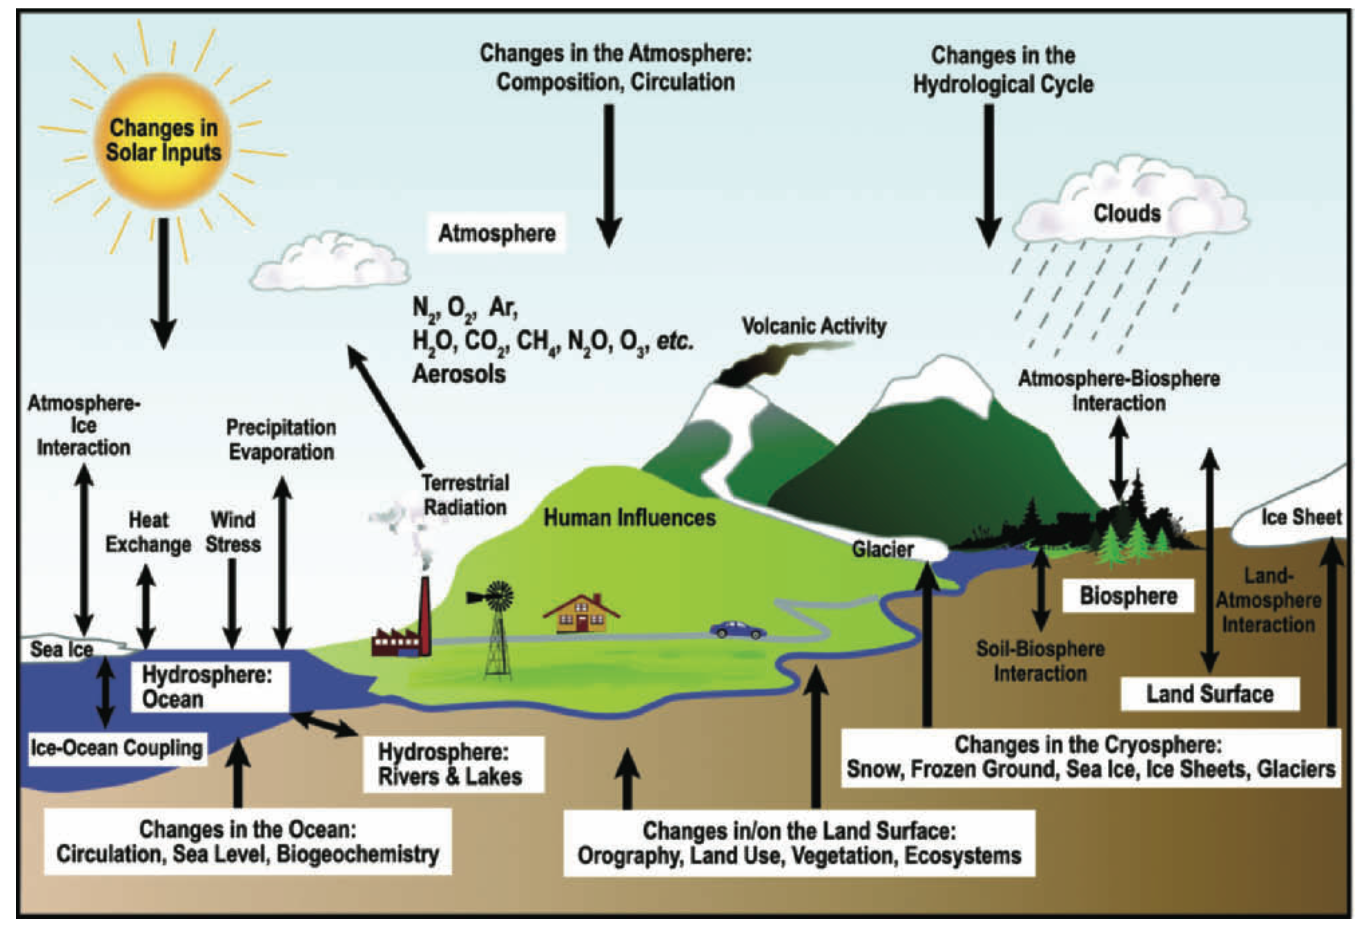
\includegraphics[width=0.7\linewidth]{images/Figure1}
			\caption{Czynniki definiujące i wpływające na klimat}
		\end{center}
	\end{figure}
\end{frame}

















\begin{frame}
\frametitle{Blocks of Highlighted Text}
\begin{block}{Block 1}
Lorem ipsum dolor sit amet, consectetur adipiscing elit. Integer lectus nisl, ultricies in feugiat rutrum, porttitor sit amet augue. Aliquam ut tortor mauris. Sed volutpat ante purus, quis accumsan dolor.
\end{block}

\begin{block}{Block 2}
Pellentesque sed tellus purus. Class aptent taciti sociosqu ad litora torquent per conubia nostra, per inceptos himenaeos. Vestibulum quis magna at risus dictum tempor eu vitae velit.
\end{block}

\begin{block}{Block 3}
Suspendisse tincidunt sagittis gravida. Curabitur condimentum, enim sed venenatis rutrum, ipsum neque consectetur orci, sed blandit justo nisi ac lacus.
\end{block}
\end{frame}

%------------------------------------------------

\begin{frame}
\frametitle{Multiple Columns}
\begin{columns}[c] % The "c" option specifies centered vertical alignment while the "t" option is used for top vertical alignment

\column{.45\textwidth} % Left column and width
\textbf{Heading}
\begin{enumerate}
\item Statement
\item Explanation
\item Example
\end{enumerate}

\column{.5\textwidth} % Right column and width
Lorem ipsum dolor sit amet, consectetur adipiscing elit. Integer lectus nisl, ultricies in feugiat rutrum, porttitor sit amet augue. Aliquam ut tortor mauris. Sed volutpat ante purus, quis accumsan dolor.

\end{columns}
\end{frame}


\begin{frame}
\frametitle{Theorem}
\begin{theorem}[Mass--energy equivalence]
$E = mc^2$
\end{theorem}
\end{frame}


\begin{frame}
\frametitle{References}
\footnotesize{
\begin{thebibliography}{99} % Beamer does not support BibTeX so references must be inserted manually as below
\bibitem[Smith, 2012]{p1} John Smith (2012)
\newblock Title of the publication
\newblock \emph{Journal Name} 12(3), 45 -- 678.
\end{thebibliography}
}
\end{frame}


\begin{frame}
\Huge{\centerline{The End}}
\end{frame}


\end{document} 